\documentclass[landscape,a0paper]{baposter}


\tracingstats=2

\usepackage{url}
\usepackage{calc}

\usepackage{amsmath}
\usepackage{amssymb}
\usepackage{relsize}
\usepackage{multirow}
\usepackage{bm}
\usepackage{tikz}
\usepackage{pgfplots}
\usepackage{caption2}
\usepackage{float} 
\usepackage{subfigure}
\usepackage{hyperref}


\usepackage{graphicx}
\usepackage{multicol}
\usepackage[fontsize=8.5pt]{fontsize}

\usepackage{pgfbaselayers}
\pgfdeclarelayer{background}
\pgfdeclarelayer{foreground}
\pgfsetlayers{background,main,foreground}
\usepackage{wrapfig}

\usepackage{times}
\usepackage{helvet}
\usepackage{palatino}


\selectcolormodel{cmyk}

%\graphicspath{{images/}}

%%%%%%%%%%%%%%%%%%%%%%%%%%%%%%%%%%%%%%%%%%%%%%%%%%%%%%%%%%%%%%%%%%%%%%%%%%%%%%%%
%%%% Some math symbols used in the text
%%%%%%%%%%%%%%%%%%%%%%%%%%%%%%%%%%%%%%%%%%%%%%%%%%%%%%%%%%%%%%%%%%%%%%%%%%%%%%%%
% Format 

\renewcommand{\Pr}{\mbox{P}}
\newcommand{\e}{\mbox{e}}
\newcommand{\dx}{\,\mbox{d}x}


%%%%%%%%%%%%%%%%%%%%%%%%%%%%%%%%%%%%%%%%%%%%%%%%%%%%%%%%%%%%%%%%%%%%%%%%%%%%%%%%
% Multicol Settings
%%%%%%%%%%%%%%%%%%%%%%%%%%%%%%%%%%%%%%%%%%%%%%%%%%%%%%%%%%%%%%%%%%%%%%%%%%%%%%%%
\setlength{\columnsep}{0.7em}
\setlength{\columnseprule}{0mm}


%%%%%%%%%%%%%%%%%%%%%%%%%%%%%%%%%%%%%%%%%%%%%%%%%%%%%%%%%%%%%%%%%%%%%%%%%%%%%%%%
% Save space in lists. Use this after the opening of the list
%%%%%%%%%%%%%%%%%%%%%%%%%%%%%%%%%%%%%%%%%%%%%%%%%%%%%%%%%%%%%%%%%%%%%%%%%%%%%%%%
\newcommand{\compresslist}{%
\setlength{\itemsep}{1pt}%
\setlength{\parskip}{0pt}%
\setlength{\parsep}{0pt}%
}


%%%%%%%%%%%%%%%%%%%%%%%%%%%%%%%%%%%%%%%%%%%%%%%%%%%%%%%%%%%%%%%%%%%%%%%%%%%%%%
%%% Begin of Document
%%%%%%%%%%%%%%%%%%%%%%%%%%%%%%%%%%%%%%%%%%%%%%%%%%%%%%%%%%%%%%%%%%%%%%%%%%%%%%

\begin{document}


%%%%%%%%%%%%%%%%%%%%%%%%%%%%%%%%%%%%%%%%%%%%%%%%%%%%%%%%%%%%%%%%%%%%%%%%%%%%%%
%%% Here starts the poster
%%%---------------------------------------------------------------------------
%%% Format it to your taste with the options
%%%%%%%%%%%%%%%%%%%%%%%%%%%%%%%%%%%%%%%%%%%%%%%%%%%%%%%%%%%%%%%%%%%%%%%%%%%%%%
% Define some colors
\definecolor{silver}{cmyk}{0,0,0,0.3}
\definecolor{yellow}{cmyk}{0,0,0.9,0.0}
\definecolor{reddishyellow}{cmyk}{0,0.22,1.0,0.0}
\definecolor{black}{cmyk}{0,0,0.0,1.0}
\definecolor{darkYellow}{cmyk}{0,0,1.0,0.5}
\definecolor{darkSilver}{cmyk}{0,0,0,0.1}
\definecolor{lightyellow}{cmyk}{0,0,0.3,0.0}
\definecolor{lighteryellow}{cmyk}{0,0,0.1,0.0}
\definecolor{lighteryellow}{cmyk}{0,0,0.1,0.0}
\definecolor{lightestyellow}{cmyk}{0,0,0.05,0.0}
\definecolor{cyan}{cmyk}{1,0,0,0}
\definecolor{lightcyan}{cmyk}{0.5,0,0,0}
\definecolor{pastelcyan}{cmyk}{0.25,0,0,0}
\definecolor{magenta}{cmyk}{0,1,0,0}
\definecolor{yellow}{cmyk}{0,0,1,0}
\definecolor{lightyellow}{cmyk}{0,0,0.5,0}
\definecolor{pastelyellow}{cmyk}{0,0,0.25,0}
\definecolor{black}{cmyk}{0,0,0,1}
\definecolor{darkgray}{cmyk}{0,0,0,0.75}
\definecolor{gray}{cmyk}{0,0,0,0.5}
\definecolor{lightgray}{cmyk}{0,0,0,0.25}
\definecolor{white}{cmyk}{0,0,0,0}
\definecolor{red}{cmyk}{0,1,1,0}
\definecolor{orange}{cmyk}{0,0.5,1,0}
\definecolor{scarlet}{cmyk}{0,1,0.5,0}
\definecolor{brown}{cmyk}{0.5,0.75,1,0}
\definecolor{camel}{cmyk}{0.25,0.375,0.5,0}
\definecolor{cream}{cmyk}{0,0.2,0.3,0}
\definecolor{green}{cmyk}{1,0,1,0}
\definecolor{lightgreen}{cmyk}{0.5,0,0.5,0}
\definecolor{pastelgreen}{cmyk}{0.25,0,0.25,0}
\definecolor{mossgreen}{cmyk}{0.64,0.4,1,0}
\definecolor{yellowgreen}{cmyk}{0.5,0,1,0}
\definecolor{skyblue}{cmyk}{0.4,0.16,0,0}
\definecolor{royal}{cmyk}{1.0,0.5,0,0}
\definecolor{navyblue}{cmyk}{0.9,0.75,0.5,0}
\definecolor{lightnavy}{cmyk}{0.4,0.3,0.2,0}
\definecolor{blue}{cmyk}{1,1,0,0}
\definecolor{lightblue}{cmyk}{0.5,0.5,0,0}
\definecolor{pastelblue}{cmyk}{0.25,0.25,0,0}
\definecolor{lightpastelblue}{cmyk}{0.15,0.15,0,0}
\definecolor{lightestpastelblue}{cmyk}{0.05,0.05,0,0}
\definecolor{lavender}{cmyk}{0.25,0.25,0,0}
\definecolor{violet}{cmyk}{0.75,1,0.25,0}
\definecolor{purple}{cmyk}{0.5,1,0.5,0}
\definecolor{lightpurple}{cmyk}{0.25,0.5,0.25,0}
\definecolor{pink}{cmyk}{0,0.5,0,0}



%%

\typeout{Poster Starts}
%\background{
  %\begin{tikzpicture}[remember picture,overlay]%
  %  \draw (current page.north west)+(-2em,-2em) node[anchor=north west] %{\hspace{-2em}\includegraphics[height=1.1\textheight]{silhouettes_background}};
 % \end{tikzpicture}%
%}




\newlength{\leftimgwidth}
\begin{poster}%
  % Poster Options, such as colours etc
  {
  % Show grid to help with alignment
  grid=false,
 % Column spacing
  colspacing=0.5em,
 % Color style
 % bgColorOne=pastelblue,
 %bgColorTwo=lightpastelblue,
  bgColorOne=white,
  bgColorTwo=white,
  borderColor=silver,
  headerColorOne=skyblue,
  headerColorTwo=purple,
  headerFontColor=black,
 % boxColorOne=lightpastelblue,
 % boxColorTwo=lightestpastelblue,
 boxColorOne=white,
 boxColorTwo=white,
 % Format of textbox
  textborder=roundedleft,
% textborder=rectangle,
% Format of text header
  eyecatcher=true,
  headerborder=open,
  headerheight=0.12\textheight,
  headershape=roundedright,
  headershade=plain,
  headerfont=\large\textsf, %Sans Serif
  boxshade=plain,
%  background=shade-tb,
 % background=plain,
  background=none,
  linewidth=2pt
  }
  % Eye Catcher
  {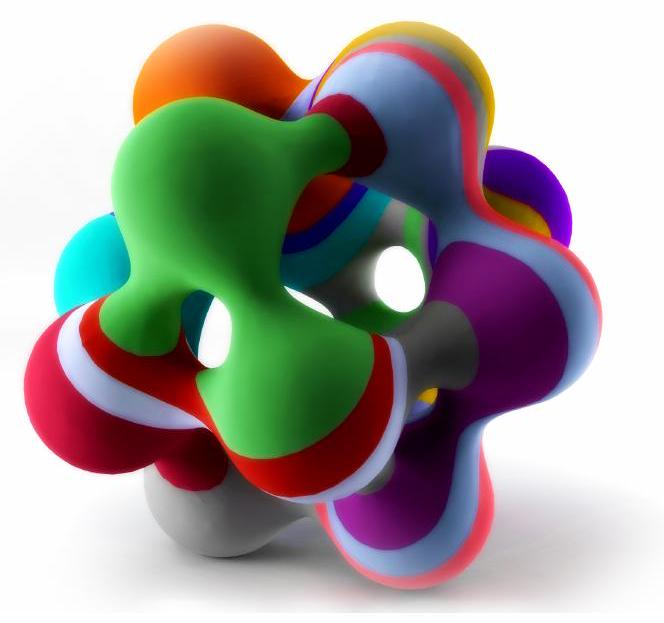
\includegraphics[width=10em]{1234.png}} % select eyecatcher=false above if not required. If no eye catcher is present, the title is left aligned.
  % Title
  {\sf %Sans Serif
  %\bf% Serif
    {\HUGE The Euler Characteristic through Morse Theory}}
  % Authors
  {\sf %Sans Serif
  % Serif
  \vspace{1em} 
  \LARGE{WHY}\\
  }
  % University logo
  { % The makebox allows the title to flow into the logo
    \makebox[8em][r]{%
        \begin{minipage}{16em}
				\hfill 
\includegraphics[height=4em]{imperial.pdf}
				\end{minipage}
      
    }
  }

  \tikzstyle{light shaded}=[top color=baposterBGtwo!30!white,bottom color=baposterBGone!30!white,shading=axis,shading angle=30]

  % Width of left inset image
     \setlength{\leftimgwidth}{0.78em+8.0em}

%%%%%%%%%%%%%%%%%%%%%%%%%%%%%%%%%%%%%%%%%%%%%%%%%%%%%%%%%%%%%%%%%%%%%%%%%%%%%%
%%% Now define the boxes that make up the poster
%%%---------------------------------------------------------------------------
%%% Each box has a name and can be placed absolutely or relatively.
%%% The only inconvenience is that you can only specify a relative position 
%%% towards an already declared box. So if you have a box attached to the 
%%% bottom, one to the top and a third one which should be in between, you 
%%% have to specify the top and bottom boxes before you specify the middle 
%%% box.
%%%%%%%%%%%%%%%%%%%%%%%%%%%%%%%%%%%%%%%%%%%%%%%%%%%%%%%%%%%%%%%%%%%%%%%%%%%%%%
    %
    % A coloured circle useful as a bullet with an adjustably strong filling
\newcommand{\colouredcircle}[1]{%
      \tikz{\useasboundingbox (-0.2em,-0.32em) rectangle(0.2em,0.32em); \draw[draw=black,fill=baposterBGone!80!black!#1!white,line width=0.03em] (0,0) circle(0.18em);}}

%%%%%%%%%%%%%%%%%%%%%%%%%%%%%%%%%%%%%%%%%%%%%%%%%%%%%%%%%%%%%%%%%%%%%%%%%%%%%%
  \headerbox{Abstract}{name=abstract,column=0,row=0}{This poster introduce the Morse theory and its application in the computation of the Euler characteristic of a manifold. It also gives a intuitive way to understand Poincar\'e duality by Morse Lemma. This poster assumes the knowledge of basic algebraic topology.
 }

%%%%%%%%%%%%%%%%%%%%%%%%%%%%%%%%%%%%%%%%%%%%%%%%%%%%%%%%%%%%%%%%%%%%%%%%%%%%%%


%%%%%%%%%%%%%%%%%%%%%%%%%%%%%%%%%%%%%%%%%%%%%%%%%%%%%%%%%%%%%%%%%%%%%%%%%%%%%%
  \headerbox{Introduction to Morse Theory}{name=sample,column=0,below=abstract}{
%%%%%%%%%%%%%%%%%%%%%%%%%%%%%%%%%%%%%%%%%%%%%%%%%%%%%%%%%%%%%%%%%%%%%%%%%%%%%%
\begin{wrapfigure}{r}{2.665cm}
  \centering
  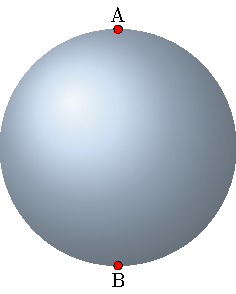
\includegraphics[width=0.175\textwidth]{spere.pdf}
  \caption{Sphere}
  \centering
  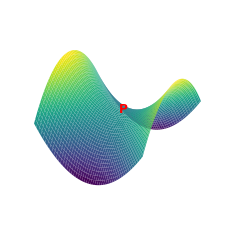
\includegraphics[width=0.3\textwidth]{saddle_surface.png}
  \caption{Saddle surface}
  \end{wrapfigure}
Morse theory is to study the topology of a manifold $M$ by 
analyzing the critical points of a smooth function $f:M\rightarrow \mathbb{R}$. 
The function $f$ is called a \textbf{Morse function} if all of its critical points are 
non-degenerate. The classical instance is to consider the height function 
defined on a spere $S^2$ illustrated in Figure $1$, which is a Morse 
function with two critical points $A$ and $B$, a maximum and a minimum, and we notice 
that moving upward along the value of the function, the level sets all have the same 
topology until we reach the critical points.
Another important aspect of Morse theory is the \textbf{Morse lemma} which states: Let $f:M \to \mathbb{R}$ be a Morse function and $p$ be a non-degenerate critical point of $f$. Then there exists a chart (called a \textbf{Morse chart}) $(x_1,\ldots, x_n)$ around $p$ such that, on the chart
$$
f(x)=f(x_1,\ldots, x_n)=f(p)-\sum_{j=1}^{i}x_j^2+\sum_{j=i+1}^{n}x_j^2
$$
where $i$ is the \textbf{index} of $p$.
 In 2 or 3 dimensions, the index 
 can be understood intuitively as the number of "linearly independent decreasing directions" 
 at a critical point. For instance, consider a Morse function defined on the 
 saddle surface shown in Figure 2. The index of $P$ is $1$, indicating a single 
 linearly independent decreasing direction.
}

\headerbox{Pseudo-gradient and CW complex}{name=cc, column = 0, above = bottom}{
  \textbf{Definition: (Pseudo-gradient)}: Let $f: M \to \mathbb{R}$ be a Morse function. A pseudo-gradient adapted to $f$ is a \textbf{vector field}  $X$ on $M$ such that:
\begin{itemize}\compresslist
  \item $<\nabla_x f, X_x> \leq 0$($ < > $ denotes inner product), where equality holds if and only if $x$ is a critical point of $f$.
  \item In a Morse chart around a critical point $x$, $X$ agrees with $-\nabla f$ for the canonical metric on $\mathbb{R}^n$.
\end{itemize} The vector flows of $X$ are called \textbf{trajectories} of $X$ flowing from the region of high values towards the region of low values and connecting the critical points.\\
\textbf{Definition (CW complex)}:A CW complex is a topological space built by attaching cells of different dimensions along their boundaries. }

%%%%%%%%%%%%%%%%%%%%%%%%%%%%%%%%%%%%%%%%%%%%%%%%%%%%%%%%%%%%%%%%%%%%%%%%%%%%%%
\headerbox{Morse complex and Morse Homology}{name=mm,column=1,span = 2,row = 0}{
\textbf{Definition (Morse complex)}: Let $f: M \to \mathbb{R}$ be a Morse function, $\text{Crit}_k(f)$ denote the set of critical points $c_k$ of $f$ and $n_X(c_{k+1},c_k)$ be the number of the trajectories of $X$ going from $c_{k+1}$ to $c_k$. The Morse complex of $f$ is a complex defined as:
$$
\cdots \rightarrow C_{k+1}(f, R) \xrightarrow{\partial_{k+1}} C_k(f, R) \xrightarrow{\partial_k} C_{k-1}(f,R) \rightarrow \cdots
$$
where  $C_k(f,R) = \left\{ \sum_{c\in \text{Crit}_k(f)} a_c c \mid a_c \in R \right\} $ for some ring $R$ and the 
\textbf{boundary map} $\partial_{k+1}:C_{k+1}(f,R) \to \partial_{k}(f,R)$ as $\partial(c_{k+1})=\sum_{c\in \text{Crit}_k(f)} n_X(c_{k+1},c_k)c_k$ where $n_X(c_{k+1},c_k)$ denotes the number of trajectories of $X$ going from $c_{k+1}$ to $c_k$. The Morse complex could form a CW complex if the pseudo-gradient $X$ satifying the \textbf{Smale condition}: if all stable and unstable manifolds intersect transversally.\\
\textbf{Definition($k$-th Morse Homology group)}: The $k$-th Morse Homology group is the quotient $H_k(f, R) = \text{Ker}\partial_{k}/\text{Im}\partial_{k+1}$ and we name $\dim H_k(f, R)$ as \textbf{Betti number} $b_k(M)$. For the the height function $h$ defined on the "sphere" in Figure $3$, it has $4$ critical points, one of index $0(a)$, one of index $1(b)$, and two of index $2(c,d)$. By the definitions above, we find that for the Morse homology of the "sphere"  $H_k(h, \mathbb{Z}/2\mathbb{Z}) = \mathbb{Z}/ 2\mathbb{Z}$ for $k \in \{0,n\}$ but $0$ otherwise, which is a \textbf{$2$ mod Morse homology}.  For the Klein bottle as depicted in Figure $4$, we can attain the \textbf{integral Morse homology} of it $H_k(h,\mathbb{Z}) = \mathbb{Z}\oplus\mathbb{Z}/2\mathbb{Z}$ for $k=1$,  $\mathbb{Z}$ for $k=0$ and $0$ otherwise. Furthermore,  A \textbf{Reeb graph} could be described by Morse function $f$ as the nodes correspond to the critical sets of $f^{-1}(c)$ and edges meet at the nodes reflects the change in topology of the level set $f^{-1}(t)$ as $t$ pass through the critical point $c$. For instance, the Reeb graph of the height function on a torus is depicted in Figure $5$.
\begin{figure}[H]
  \centering 
  \begin{minipage}[b]{0.3\textwidth} 
  \centering %图片局部居中
  \includegraphics[width=0.5\textwidth]{sphere.jpeg}
  \caption{"Sphere"}
  \end{minipage}
  \begin{minipage}[b]{0.3\textwidth} %所有minipage宽度之和要小于1,否则会自动变成竖排
  \centering %图片局部居中
  \includegraphics[width=0.3\textwidth]{Klevin.jpeg}%此时的图片宽度比例是相对于这个minipage的,不是全局
  \caption{Klein bottle}
  \end{minipage}
  \begin{minipage}[b]{0.31\textwidth} %所有minipage宽度之和要小于1,否则会自动变成竖排
    \centering %图片局部居中
    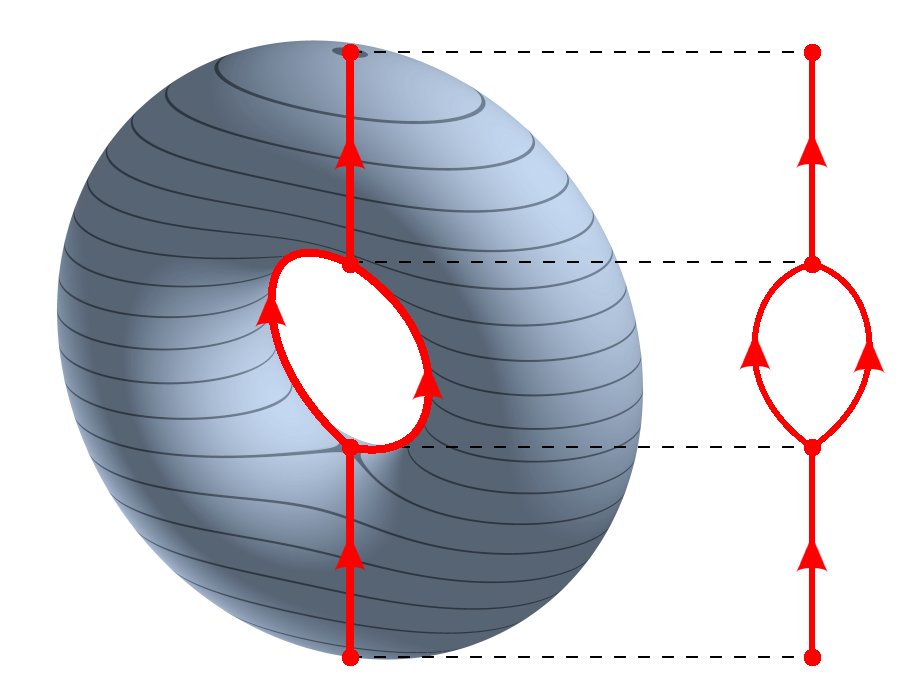
\includegraphics[width=0.67\textwidth]{reebgraph_3.png}%此时的图片宽度比例是相对于这个minipage的,不是全局
    \caption{Reeb graph of a torus}
  \end{minipage} 
  \end{figure}
}
  \headerbox{Euler Characteristic}{name=EC,column=1, span = 2, above = bottom}{The \textbf{Euler characteristic} $\chi(M)$ of a manifold $M$ is defined as $\chi(M) = \sum_{k=0}^n (-1)^k b_k(M)$.
   Next, we will prove the following equation only using rank-nullity theorem and basic algebra:
    $$
    \chi(M) = \sum_{k=0}^n (-1)^k b_k(M) = \sum_{k=0}^n (-1)^k \dim C_k(f) 
    $$
\textbf{Proof}: Let us consider the following Morse complex associated with some manifold $M$:
$$
 0 \xrightarrow{\partial_{n+1}} C_n(f) \xrightarrow{\partial_n} C_{n-1}(f) \rightarrow \cdots \rightarrow C_1(f) \xrightarrow{\partial_1} C_0(f) \xrightarrow{\partial_0} 0
$$

 $C_k(f)$ are vector spaces connected by the  boundary maps $\partial_k$ which is a linear map, then the rank-nullity theorem gives that $\dim \ker \partial_k + \dim \text{Im} \partial_k = \dim C_k(f)$. Hence,
$$
 \sum_{k=0}^n (-1)^k \dim C_k(f) = \sum_{k=0}^n (-1)^k [\dim \text{Ker} \partial_k + \dim \text{Im} \partial_k] = \sum_{k=0}^n (-1)^k [\dim \text{Ker} \partial_k - \dim \text{Im} \partial_{k+1}] = \sum_{k=0}^n (-1)^k b_k(M)
$$
It tells us that the homology is independent of the choice of Morse function. Furthermore,  if we define $\#\text{Crit}(f)$ to be the total number of the critical points of $f$, then we have
$$
  \#\text{Crit}(f) = \sum_{k=0}^n [\dim \ker \partial_k + \dim \text{Im} \partial_{k+1}] 
  \geq \sum_{k=0}^n [\dim \ker \partial_k - \dim \text{Im} \partial_{k+1}] = \sum_{k=0}^n b_k(M)
$$
The inequality holds since $\dim \text{Im} \partial_{k+1} \geq 0$. This is called \textbf{Morse Inequality}, stating that the number of critical points of a Morse function is at least equal to the sum of the Betti numbers of the manifold.
    }
     \headerbox{The Poincar\'e Duality}{name=ex,column=3}{
    By Morse Lemma, the critical points of index $k$ of $f$ are the critical points of index $n-k$ of $-f$. Then,  $C_{n-k}(-f)$ is isomorphic to $C_k(f)$ since they have have the same basis. We will get a complex of $C_{n-k+1}(-f)$ and  have the following results called the \textbf{Poincar\'e Duality}, which states that for a closed oriented $n$-manifold $M$, $b_k(M) = b_{n-k}(M)$. It was first proposed by Henri  Poincar\'e (Figure $6$)  in $1893$. It can be observed that a triangulated manifold provides insight into the existence of a dual polyhedral decomposition. This decomposition is a collection of cells, where each $k$-cell in the dual polyhedral decomposition corresponds uniquely with an $(n-k)$-cell in the original triangulation. This generalizes the concept of dual polyhedra, as illustrated in Figure $7$.
    \begin{figure}[H]
\centering %图片全局居中
%并排几个图,就要写几个minipage
\begin{minipage}[b]{0.45\textwidth} %所有minipage宽度之和要小于1,否则会自动变成竖排
\centering %图片局部居中
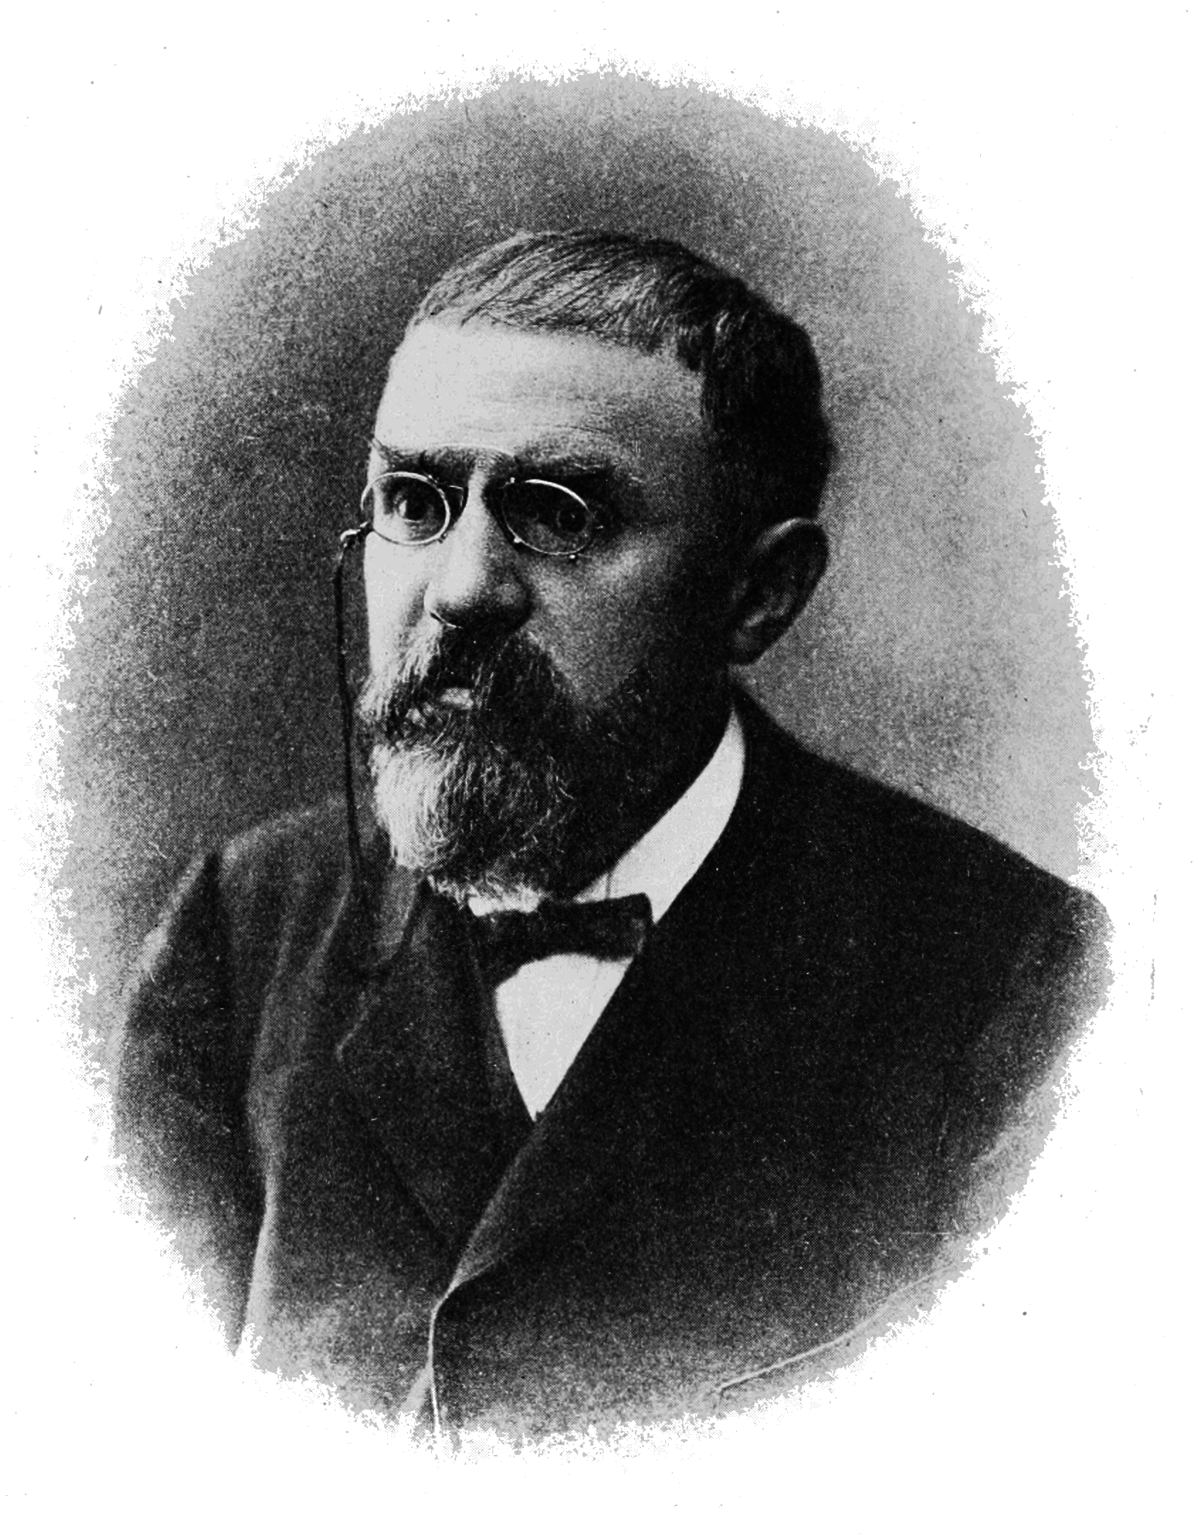
\includegraphics[width=0.5\textwidth]{Henri_Poincare.png} %此时的图片宽度比例是相对于这个minipage的,不是全局
\caption{Henri Poincar\'e}
\end{minipage}
\begin{minipage}[b]{0.45\textwidth} %所有minipage宽度之和要小于1,否则会自动变成竖排
\centering %图片局部居中
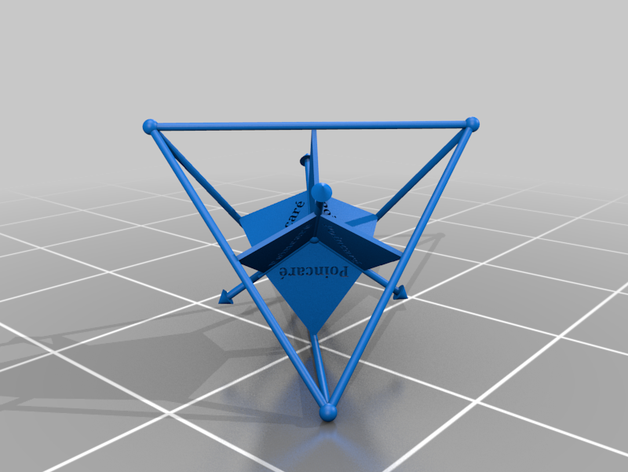
\includegraphics[width=0.8\textwidth]{PD.png}%此时的图片宽度比例是相对于这个minipage的,不是全局
\caption{Dual polyhedral decomposition}
\end{minipage}
\end{figure}
    }

  \headerbox{One Example}{name=Po,column=3,below = ex}{
Euler characteristic of sphere $S^n$ can calculateed as $\chi(S^n) = 1+(-1)^n$ by before sections. As an instance, we can consider a $2$-D sphere as shown in Figure $8$, whose Euler characteristic can be gained by apply the "Euler's polyhedral formula" to a cube as depicted in Figure $9$  since they are topological equivalent to each other: $\chi(S^2)= \chi(C) = V-E+F = 8 - 12 +6 =2 $. This is the same as the result that we calculate by Morse theory. Furthermore, by Poincar\'e Duality, the Euler characteristic of a compact manifold of odd dimension without boundary is $0$ since the terms in the alternating sum cancel each other in pairs.
      \begin{figure}[H]
\centering %图片全局居中
%并排几个图,就要写几个minipage
\begin{minipage}[b]{0.45\textwidth} %所有minipage宽度之和要小于1,否则会自动变成竖排
\centering %图片局部居中

\includegraphics[width=0.4\textwidth]{spere2.pdf} %此时的图片宽度比例是相对于这个minipage的,不是全局
\caption{A sphere}
\end{minipage}
\begin{minipage}[b]{0.45\textwidth} %所有minipage宽度之和要小于1,否则会自动变成竖排
\centering %图片局部居中
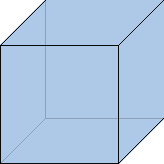
\includegraphics[width=0.4\textwidth]{square.pdf}%此时的图片宽度比例是相对于这个minipage的,不是全局
\caption{A cube}
\end{minipage}
\end{figure}
  } 
	
%%%%%%%%%%%%%%%%%%%%%%%%%%%%%%%%%%%%%%%%%%%%%%%%%%%%%%%%%%%%%%%%%%%%%%%%%%%%%%
  \headerbox{Acknowledgement and references}{name=references,column=3,above=bottom}{
   { The images of the poster are generated by Python, TikZ, and academic sources.\\
  $[1]$ Artin M \& Damian M. \emph{Morse Theory and Floer Homology}. London: Springer-Verlag; 2014\\
  $[2]$ Hatcher A. \emph{Algebraic topology}. Cambridge: Cambridge University
Press; 2001\\
  $[3]$ Milnor J. \emph{Morse theory}. Princeton: Princeton University Press; 1963\\
  }}
%%%%%%%%%%%%%%%%%%%%%%%%%%%%%%%%%%%%%%%%%%%%%%%%%%%%%%%%%%%%%%%%%%%%%%%%%%%%%%
  
\end{poster}

\end{document}